% **************************************************
% Document Class Definition
% **************************************************
\documentclass[runningheads]{llncs}

% !TEX root = main.tex
% chktex-file 46

% **************************************************
% Files' Character Encoding
% **************************************************
\PassOptionsToPackage{utf8}{inputenc}
\usepackage{inputenc}
\usepackage[ngerman,english]{babel}
\usepackage{csquotes}

% **************************************************
% Information and Commands for Reuse
% **************************************************
\newcommand{\thesisTitle}{Spectral Graph Approximation}
\newcommand{\thesisName}{Clemens Damke}
\newcommand{\thesisMatNr}{7011488}
\newcommand{\thesisSubject}{Seminar paper}
\newcommand{\thesisDate}{}

\newcommand{\thesisSupervisor}{Vitalik Melnikov}

\newcommand{\thesisUniversity}{Paderborn University}
\newcommand{\thesisUniversityDepartment}{Department of Computer Science}
\newcommand{\thesisUniversityInstitute}{Heinz Nixdorf Institute}
\newcommand{\thesisUniversityGroup}{Intelligent Systems and Machine Learning Group (ISG)}
\newcommand{\thesisUniversityCity}{Paderborn}
\newcommand{\thesisUniversityStreetAddress}{Warburger Straße 100}
\newcommand{\thesisUniversityPostalCode}{33098}



% **************************************************
% Debug LaTeX Information
% **************************************************
%\listfiles


% **************************************************
% Load and Configure Packages
% **************************************************
\usepackage{geometry}
\geometry{
  a4paper,
  % textwidth=13cm,
  % textheight=23cm,
  % heightrounded,   % integer number of lines
  hratio=1:1,      % horizontally centered
  % vratio=1:1,      % vertically centered
}
\renewcommand{\baselinestretch}{1.15}
\usepackage[parfill]{parskip}
\usepackage{float}

% Colors:
\usepackage[usenames, dvipsnames, svgnames, table]{xcolor}

\definecolor{schwarz}{HTML}{000000}
\definecolor{blau}{HTML}{3F6DB1}
\definecolor{rot}{HTML}{EE7993}
\definecolor{gruen}{HTML}{3FB17D}

\usepackage{mathtools}
\usepackage{bm}
\usepackage{bbm}
\usepackage{units}
\usepackage{upgreek}
\newcommand\numberthis{\addtocounter{equation}{1}\tag{\theequation}}

\usepackage{algorithm}
\usepackage[noend]{algpseudocode}

\usepackage{graphicx}
\usepackage{tikz}
\usetikzlibrary{arrows,positioning}
\usetikzlibrary{calc}
\newcommand{\tikzmark}[1]{\tikz[overlay,remember picture] \node (#1) {};} % chktex 1
\usepackage[labelfont=bf]{caption}
\usepackage{subcaption}
\usepackage{wrapfig}

\usepackage{pgfplots}
\usepackage{pgfplotstable}
\pgfplotsset{compat=1.14}
\usepgfplotslibrary{dateplot, statistics}
\pgfplotsset{
    cycle list={blau\\rot\\gruen\\schwarz\\},
}

\usepackage{listings}
\lstset{basicstyle=\ttfamily,breaklines=true}
\usepackage[inline]{enumitem}

\usepackage{amsmath,amssymb}
\usepackage{stmaryrd}
\usepackage{multicol}
\usepackage{pbox}
\usepackage{longtable}
\usepackage{booktabs}
\usepackage{csvsimple}
\usepackage{siunitx}

\usepackage{hyperref}
\hypersetup{% setup the hyperref-package options
    pdftitle={\thesisTitle},    %   - title (PDF meta)
    pdfsubject={\thesisSubject},%   - subject (PDF meta)
    pdfauthor={\thesisName},    %   - author (PDF meta)
    plainpages=false,           %   -
    colorlinks=false,           %   - colorize links?
    pdfborder={0 0 0},          %   -
    breaklinks=true,            %   - allow line break inside links
    bookmarksnumbered=true,     %
    bookmarksopen=true          %
}
\usepackage[nameinlink]{cleveref}
\newcommand{\crefrangeconjunction}{--}

\usepackage[						% use biblatex for bibliography
	backend=bibtex,					% 	- use biber backend (bibtex replacement) or bibtex
	style=numeric,					% 	- use alphabetic (or numeric) bib style
	natbib=true,					% 	- allow natbib commands
	hyperref=true,					% 	- activate hyperref support
	backref=true,					% 	- activate backrefs
	isbn=false,						% 	- don't show isbn tags
	url=false,						% 	- don't show url tags
	doi=false,						% 	- don't show doi tags
	urldate=long,					% 	- display type for dates
	maxnames=3,%
	minnames=1,%
	maxbibnames=5,%
	minbibnames=3,%
	maxcitenames=2,%
	mincitenames=1%
]{biblatex}
\bibliography{bib-refs}

\DeclareCiteCommand{\citenum}
  {}
  {\bibhyperref{\printfield{labelnumber}}}
  {}
  {}


\newcommand{\Dtrain}{\mathcal{D}_{\mathit{train}}}
\newcommand{\Dvalid}{\mathcal{D}_{\mathit{valid}}}
\newcommand{\Dtest}{\mathcal{D}_{\mathit{test}}}
\newcommand{\sourceinline}[2][source]{{\scriptsize\textsc{#1:~\cite{#2}}}}
\newcommand{\source}[2][source]{\null\hfill\sourceinline[#1]{#2}}

% **************************************************
% Document CONTENT
% **************************************************
\begin{document}

% --------------------------
% Front matter
% --------------------------
% !TEX root = ../main.tex
%

\title{\thesisTitle}
\author{\thesisName}
\institute{{\thesisUniversityGroup} \\
{\thesisUniversityInstitute} \\
{\thesisUniversity} \\
{\thesisUniversityStreetAddress} \\
\thesisUniversityPostalCode\ \thesisUniversityCity}

\maketitle

% !TEX root = ../main.tex
%
\begin{abstract}%
	This paper describes how coarsening affects the spectrum of a graph.
	For this the notion of restricted spectral similarity is introduced.
	This similarity measure compares graphs via the distance between their Laplacian's eigenvalues.
	The measure is used to show that the spectral distortion introduced by coarsening is smallest for regular graphs.
\end{abstract}


% --------------------------
% Body matter
% --------------------------

% !TEX root = ../main.tex
% chktex-file 21
% chktex-file 46
\section{Introduction}%
\label{sec:intro}

\pagenumbering{arabic}			% arabic page numbering
\setcounter{page}{1}			% set page counter

With the rise of Big Data applications over the recent years, working with large graph structures also became more important.
Algorithms like PageRank or spectral clustering are commonly used to analyze the web graph or social networks.
In order to run such algorithms on large graphs however, optimizations are required.

For this purpose we will specifically look at \textit{graph coarsening}.
Coarsening reduces the size of a given graph while preserving its overall structure via some notion of graph similarity that will be defined later.
Graph algorithms can then be run on the smaller coarsened graph.
Afterwards the result for the coarsened graph can be iteratively refined to obtain an approximate result for the original graph.
\Cref{fig:intro:overview} illustrates this approach.
\begin{figure}[ht]
	\centering
	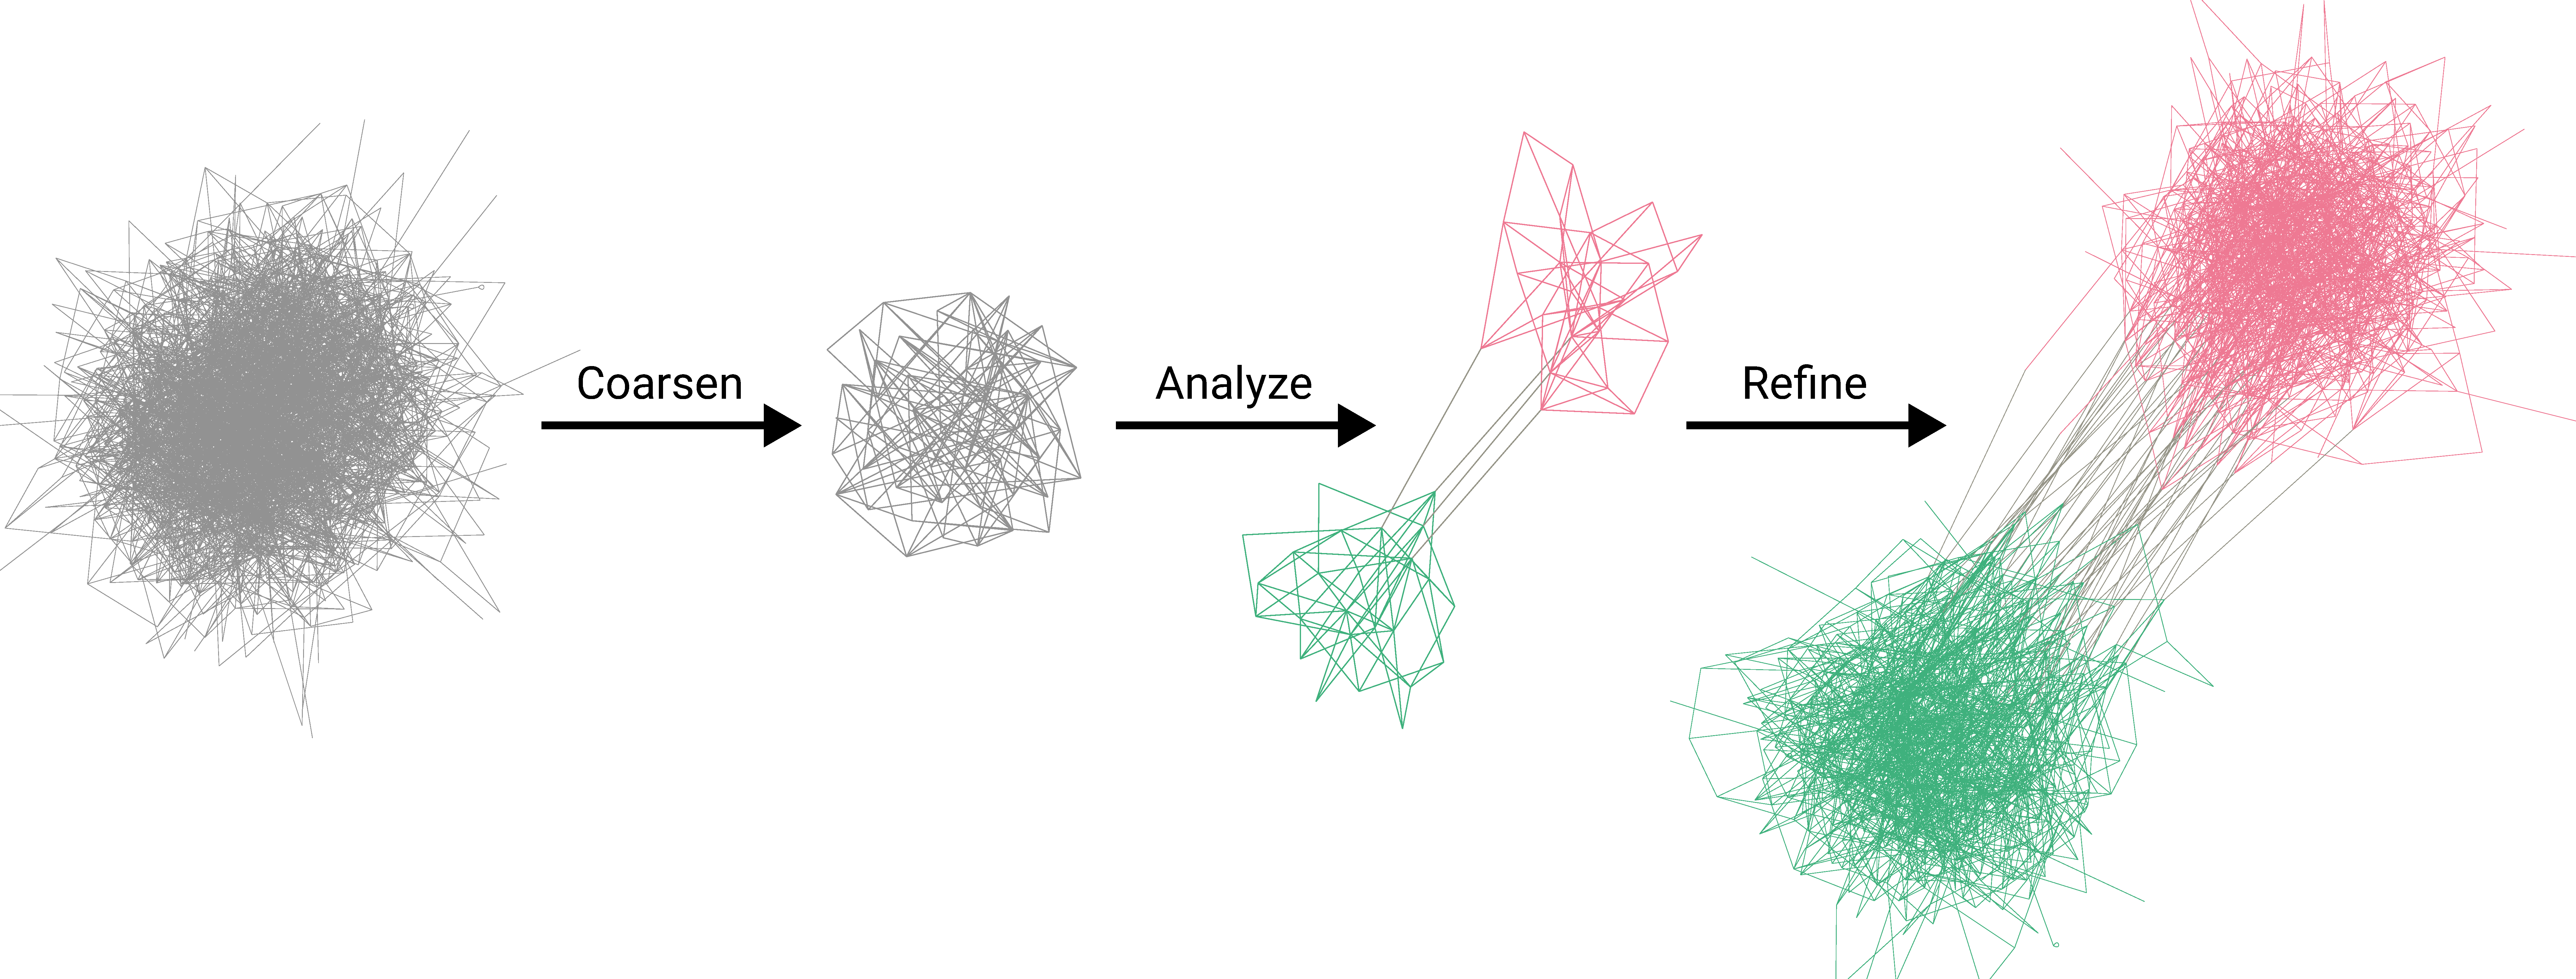
\includegraphics[width=0.8\linewidth]{gfx/intro/overview.pdf}
	\caption{%
		Using graph coarsening to speed up graph algorithms, e.g.\  Min-Cut.
	}\label{fig:intro:overview}
\end{figure}

The goal of this paper is to show how graph coarsening works and how it affects the results of graph algorithms.
This introduction consists of three sections, each of which aims to answer one main question:
\begin{enumerate}
	\item \textit{How can the structural properties of a graph be formally described?}
		To describe graph coarsening and its effects, the similarity between a graph $G$ and its coarsened version $G_c$ has to be quantified.
		We begin with an introduction to spectral graph theory.
		It allows us to describe the structure of graphs and provides the notion of the \textit{graph spectrum}, a way to describe the overall structure of graphs.
	\item \textit{How does graph coarsening work?}
		Based on the notion of the graph spectrum, we will formally define the graph coarsening operation and describe a randomized coarsening algorithm.
	\item \textit{How does coarsening affect the result of graph algorithms?}
		Finally we will put bounds on how much the described coarsening algorithm is expected to increase the error of the spectral clustering algorithm.
\end{enumerate}

% !TEX root = ../main.tex
% chktex-file 21
\section{Spectral Graph Theory}%
\label{sec:sgt}

\subsection{Extending the Fourier Transform to Graphs}%
\label{sec:sgt:spec}

TODO

% !TEX root = ../main.tex
% chktex-file 21
% chktex-file 46
\section{Graph Coarsening}%
\label{sec:coarse}

We will now see how the size of a graph $G$ can be reduced via \textit{graph coarsening}.
The resulting coarsened graph $G_c$ should ideally be structurally similar to $G$, i.e.\  it should have a similar spectrum.
In this section we will first define the class of coarsening operators $C$ and give an intuition on how they change the shape of a graph.
Then we will describe a randomized algorithm to compute such a coarsening.

\subsection{Definition of the Coarsening Operator}%
\label{sec:coarse:formal}

The core idea of graph coarsening is to replace clusters of vertices in the original graph $G$ by single vertices in the coarsened graph $G_c$.
Formally this means that the original vertices $\mathcal{V} = \{ v_1, \dots, v_N \}$ are mapped to a smaller vertex set $\mathcal{V}_c = \{ v'_1, \dots, v'_n \}$ via a surjective mapping $\varphi: \mathcal{V} \to \mathcal{V}_c$.
The original edges $(v_i, v_j) \in \mathcal{E}$ are mapped to $(\varphi(v_i), \varphi(v_j))$, resulting in a reduced edge set $\mathcal{E}_c$ that contains every edge for which $\varphi(v_i) \neq \varphi(v_j)$.
\Cref{fig:coarse:example:original,fig:coarse:example:coarsened} show an exemplary graph coarsening.
To reverse the coarsening mapping, we define $\varphi^{-1}: \mathcal{V}_c \to \mathcal{P}(\mathcal{V})$ as the mapping from a coarsened vertex to the set of original vertices it represents.
\begin{figure}[ht]
	\centering
	\begin{subfigure}{0.33\textwidth}
		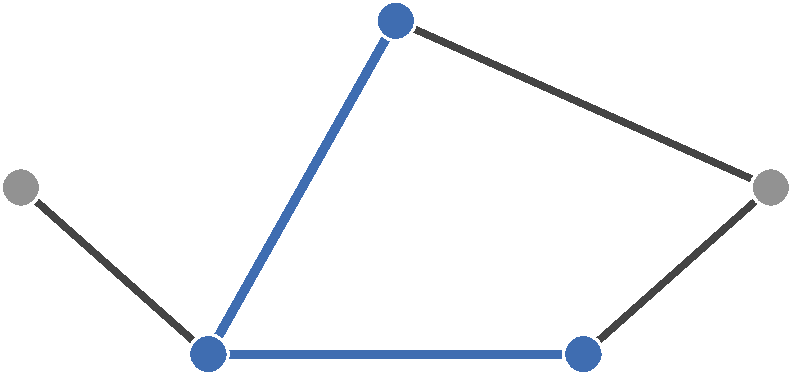
\includegraphics[width=0.9\linewidth]{gfx/coarse/example/original.pdf}
		\caption{Original $G$}\label{fig:coarse:example:original}
	\end{subfigure}%
	\begin{subfigure}{0.33\textwidth}
		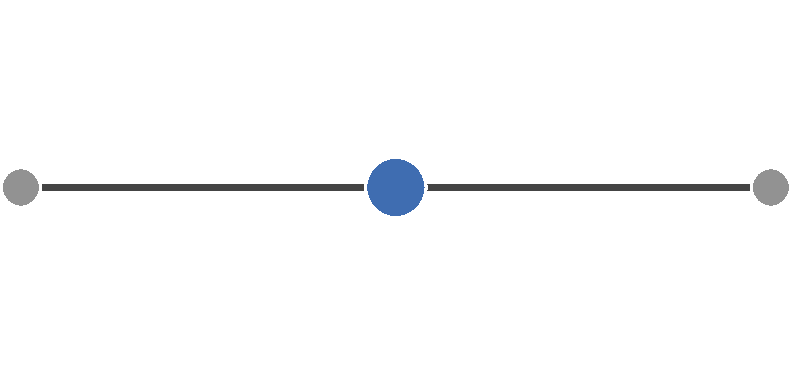
\includegraphics[width=0.9\linewidth]{gfx/coarse/example/coarsened.pdf}
		\caption{Coarsened $G_c$}\label{fig:coarse:example:coarsened}
	\end{subfigure}%
	\begin{subfigure}{0.33\textwidth}
		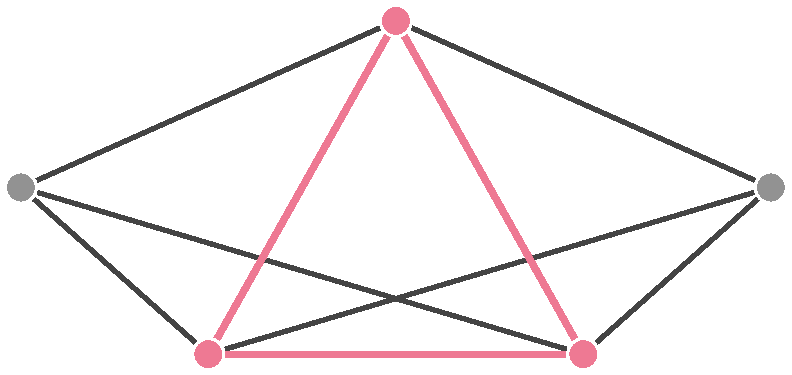
\includegraphics[width=0.9\linewidth]{gfx/coarse/example/reexpanded.pdf}
		\caption{Approximated $\widetilde{G}$}\label{fig:coarse:example:reexpanded}
	\end{subfigure}
	\caption{%
		Example showing the effect of coarsening $G$ when merging the blue vertices into a single vertex.
		The graph $\widetilde{G}$ on the right shows the result of re-expanding $G_c$.
	}\label{fig:coarse:example}
\end{figure}

In the last section we saw how graphs can be described via their Laplacian $L$.
Since our goal is to analyze the effects of coarsening on the overall characteristics of a graph, we will now describe a coarsening $\varphi$ as an operation that acts directly on $L$.
The so called \textit{coarsening matrix} $C \in \mathbb{R}^{n \times N}$ is essentially just a matrix representing $\varphi$:
\begin{align}
	\varphi(v_i) = v'_j \Leftrightarrow C b_i = n_j b'_j\quad
	& \text{with the standard basis vectors } b_i \in \mathbb{R}^N,\, b'_j \in \mathbb{R}^n\\
	& \text{and normalization factor\footnotemark\ } n_j := {\left|\varphi^{-1}(v'_j)\right|}^{-\frac{1}{2}} \nonumber
\end{align}
\footnotetext{%
	$n_j$ is required for technical reasons.
	It normalizes $\Pi = C^{\top} C$ so that it is a projector, i.e.\  so it has eigenvalues in $\{ 0, 1 \}$.
	This ensures that $G$ and $\widetilde{G}$ have the same total weight.
}%
Analogous to $\varphi$, the coarsening matrix $C$ maps vertex basis vectors of $G$ to vertex basis vectors of $G_c$.
By linearity any signal $x \in \mathbb{R}^N$ on $G$ can thus be downsampled to a signal $x_c := C x \in \mathbb{R}^n$ on the coarsened graph $G_c$;
the signal strengths of merged vertices will simply be added up.
Similarly a downsampled signal $x_c$ can be upsampled again to an approximation $\widetilde{x} \in \mathbb{R}^N$ of the original signal $x$.
Upsampling uniformly distributes the signal strength of each $v'_j \in \mathcal{V}_c$ among $\varphi^{-1}(v'_i)$, where the inverse $\varphi^{-1}$ can be represented by $C^{\top}$:
\begin{align}
	\widetilde{x} := C^{\top} x_c = C^{\top} C x = \Pi x\quad\text{with the projector } \Pi := C^{\top} C
\end{align}

Since both the coarsening matrix $C$ and the Laplacian $L$ are operators acting on signals, we can combine them to define the \textit{coarsened Laplacian} $L_c$ and also the \textit{approximate Laplacian} $\widetilde{L}$:
\begin{align}
	L_c := C L C^{\top}\quad\text{and}\quad\widetilde{L} := C^{\top} L_c C = \Pi L \Pi
\end{align}
$L_c$ represents the Laplacian of the coarsened graph $G_c$\footnote{%
	$L_c$ is actually not a proper combinatorial Laplacian, i.e.\  its rows do not generally add up to $0$.
	To fix this, $L_c$ could be normalized, which is however not necessary for our analysis.
	We refer to \citet[Sec.~2.1]{Loukas2018} for the details.
}.
$\widetilde{L}$ represents the Laplacian of the graph $\widetilde{G}$, which is the result of re-expanding the coarsened graph $G_c$.
During re-expansion, every vertex $v'_i \in \mathcal{V}_c$ is replaced by the complete graph on the vertex set $\varphi^{-1}(v'_i)$.
The neighbors of each replaced $v'_i$ are connected to the vertices that replace it.
\Cref{fig:coarse:example:reexpanded} shows how a graph might look like after such a re-expansion.

\subsection{The Randomized Edge Contraction Algorithm}%
\label{sec:coarse:rec}

Now that we have defined the coarsening operator, we will look at a simple randomized algorithm which finds a coarsened graph $G_c$ that is spectrally similar to some given graph $G$.
The so called \textit{Randomized Edge Contraction}~(REC)~\cite{Loukas2018} algorithm is a variant of the well-known greedy algorithm for maximal matching generation.
It contracts random edges until the vertex count has been reduced by a ratio $r$ or until there are no more neighboring pairs of unmerged vertices.
The contracted edges are chosen with a probability proportional to their weight.
\begin{figure}[H]
	\setlength{\intextsep}{0pt}
	\begin{minipage}{0.6\linewidth}
		\begin{algorithm}[H]
			\caption{Randomized Edge Contraction}\label{algo:coarse:rec}
			\begin{algorithmic}[1]
				\Function{REC}{$G = (\mathcal{V}, \mathcal{E}, W), r \in [0, \frac{1}{2}]$}
					\State{$\mathcal{C} \leftarrow \mathcal{E}$, $G_c \leftarrow G$}
					\State{$Z \leftarrow \sum_{e_{i j} \in \mathcal{E}} w_{i j}$}
					\While{$|\mathcal{C}| > 0$ and $\frac{|\mathcal{V}_c|}{|\mathcal{V}|} > 1 - r$}
						\State{Select some $e_{i j} \in \mathcal{C}$ with prob.\  $p_{i j} = \frac{w_{i j}}{Z}$.}
						\State{$\mathcal{C} \leftarrow \mathcal{C} \setminus \mathcal{N}_{i j}$}
						\State{$Z \leftarrow \sum_{e_{i j} \in \mathcal{C}} w_{i j}$}
						\State{$G_c \leftarrow \mathit{contract}(G_c, e_{i j})$}
					\EndWhile{}
					\State{\Return{$G_c$}}
				\EndFunction{}
			\end{algorithmic}
		\end{algorithm}
	\end{minipage}%
	\begin{minipage}{0.4\linewidth}
		\begin{figure}[H]
			\centering
			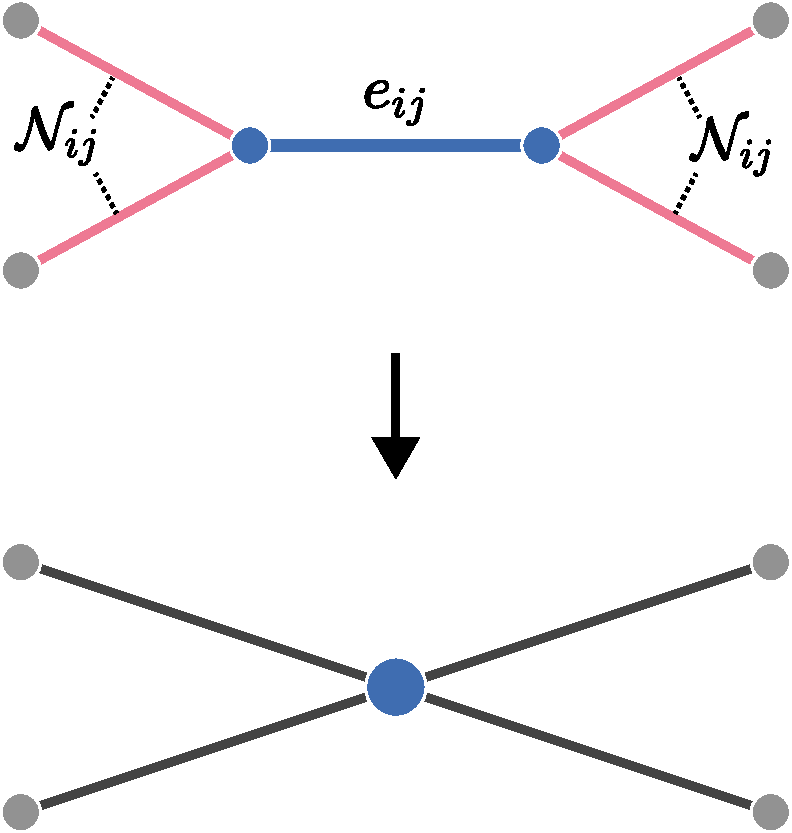
\includegraphics[width=0.75\linewidth]{gfx/coarse/rec.pdf}
			\caption{$\mathit{contract}(G_c, e_{i j})$.}\label{fig:coarse:rec}
		\end{figure}
	\end{minipage}
\end{figure}

We define the neighborhood $\mathcal{N}_{i j}$ as the set of incident edges of $e_{i j}$, including $e_{i j}$ itself;
this is shown as the red and blue edges in \cref{fig:coarse:rec}.
REC only merges vertices that have not been merged with some other vertex yet.
Thus the reduction ratio $r = \frac{N - n}{N}$ is at most $\frac{1}{2}$, i.e.\  $|\mathcal{V}_c| \geq \frac{1}{2} |\mathcal{V}|$.
If the node count needs to be further reduced, REC has to be applied multiple times.

% !TEX root = ../main.tex
% chktex-file 21
\section{Spectral Graph Similarity}%
\label{sec:ss}

TODO

% !TEX root = ../main.tex
% chktex-file 21
% chktex-file 46
\section{Conclusion}%
\label{sec:conclusion}

We have now discussed the three main topics of this paper:
\begin{enumerate*}
	\item How the structural properties of graphs can be described via spectral graph theory.
	\item How graphs can be coarsened via the REC algorithm.
	\item How to bound the effects of coarsening via RSS and what this implies for spectral clustering.
\end{enumerate*}

Based on the work we presented, there are two main open questions for future research:
\begin{enumerate*}
	\item The described RSS bound assumes a single application of the REC algorithm.
		For multiple REC applications with a total reduction ratio of $r > \frac{1}{2}$, the RSS bound still needs to be generalized.
	\item Currently the RSS bound has only been applied to the analysis of spectral clustering.
		To make the results more generally applicable, the implications for other graph algorithms, e.g.\ graph convolutional neural networks, are still to be considered.
\end{enumerate*}


% --------------------------
% Back matter
% --------------------------
{%
\renewcommand{\bibfont}{\normalfont\small}
\setlength{\biblabelsep}{5pt}
\setlength{\bibitemsep}{0.5\baselineskip plus 0.5\baselineskip} % chktex 1
\setcounter{biburllcpenalty}{9000}
\setcounter{biburlucpenalty}{9999}
\printbibliography[nottype=www]
\printbibliography[heading=subbibliography,title={Webpages},type=www]
}

% **************************************************
% End of Document CONTENT
% **************************************************
\end{document}
